%特別研究論文
\documentstyle[11pt,a4j,makeidx,ascmac,epsbox,ronbun,hyoushi,fig_tab,theorem,list,cprog,graphicx,comment]{jreport}
	\newcommand{\ve}[1]{\mbox{\boldmath{$#1$}}}
	\def\rubyfont{\tiny}
	\makeatletter
	\def\ruby#1#2{\leavevmode\vbox{%
	\baselineskip\z@skip\lineskip.25ex
	\ialign{##\crcr\rubyfont\hfill#2\hfill\crcr
	\hfill#1\hfill\crcr}}}
	\textwidth 6.5in
	\textheight 9.5in
	\oddsidemargin .2in
	\topmargin -.5in
	\parindent 1zw
	\makeindex
	
\begin{document}

\large
	%\maketitle
	%#!jlatex main.tex
{\large
\title{\Large{\underline{特別研究}}\\
\vspace{0.5cm}
伸縮センサを用いた足関節ロボットの空気圧人工筋活動計測}}
\author{丹羽 英人}
\maketitle
	\pagenumbering{roman}
	\tableofcontents\newpage
	\listoffigures\newpage
	\listoftables\newpage
	\pagebreak
	\pagenumbering{arabic}

\chapter{緒言}
\section{研究背景}
近年,少子高齢化が非常に深刻に進んでおり,リハビリテーションロボットの需要が増大している.
その様な中ヒトの運動戦略を理解することで,ヒトの運動機能への介入や調和を目指した
リハビリテーションロボットの開発がより行われやすくなると考えられている.それらの
リハビリテーションロボットの開発・実用化が行われることで,患者と相互に関わりながら
運動機能の再獲得を促すことなどが期待されている.リハビリテーションロボットは,
より効率的な効果を上げるため,ヒトの運動戦略に基づきながらトレーニングすることが望まれてる.
また,ヒトのような柔軟かつ滑らかな運動を実現することを目指す筋骨格ロボットの開発において,
ヒトの骨格や運動制御を規範としてロボットのシステムに応用することは非常に有望な方法であると
考えられている.これらのロボットの実現をするため,ヒトの骨格の仕組みや運動戦略を
明らかにすることは必要不可欠である.

また,ロボットの社会進出は凄まじさを増しており,街中でもロボットを見かける様になった.
そのような環境の中,旧来からのハードなロボットではロバスト性に限りがあり,安全性の観点からも
難が見られる.故に,伸縮性や柔軟性に優れた,ソフトロボットの研究開発が盛んに行われている.
ソフトロボットはその伸縮性や柔軟性を生かし助長性の高い,動作を行うことができるようになっている.
更に,これらに合わせて,ロボットの動作を計測するセンサも柔軟なものとなる必要性が出てきた.

本研究はこれらの研究背景の元,ヒトと同機能を持ったやわらかいアクチュエータを用いた
足関節ロボットの開発を行い,やわらかいストレッチセンサの開発を行った.

\section{先行研究例}

\subsection{フレキシブルストレッチセンサ}%TODO:ストレッチセンサのお話を書く
ロボットの社会進出に伴い,ハードなロボットではなく柔軟性を持ったやわらかロボットの研究開発が
盛んに行われている.その様な中,ロボットの動作計測を行うセンサーも柔軟性を持つ必要性が増加している.
導電性ゴムを利用したストレッチセンサの開発が行われ実際に販売されているが,高価であり既製品であるため,センサー長が
定まったもののみとなっている.\cite{bando}

soft robotics toolkit\cite{MITSoftRobot}において,シリコンと導電性布をもちいた自作できるストレッチセンサが
紹介されている.本センサは,伸縮性に優れており,柔軟性も兼ね備えたものとなっている.また,
製作コストも\$23と非常に安価なものであると紹介されている.

今回は,このような安価で自作することのできるセンサーとその計測系を作成し,
本センサーを空気圧人工筋を用いた足関節ロボットに搭載し,空気圧人工筋の伸展の計測を行うことを目標とする.
\begin{figure}[h]
    \begin{center}
        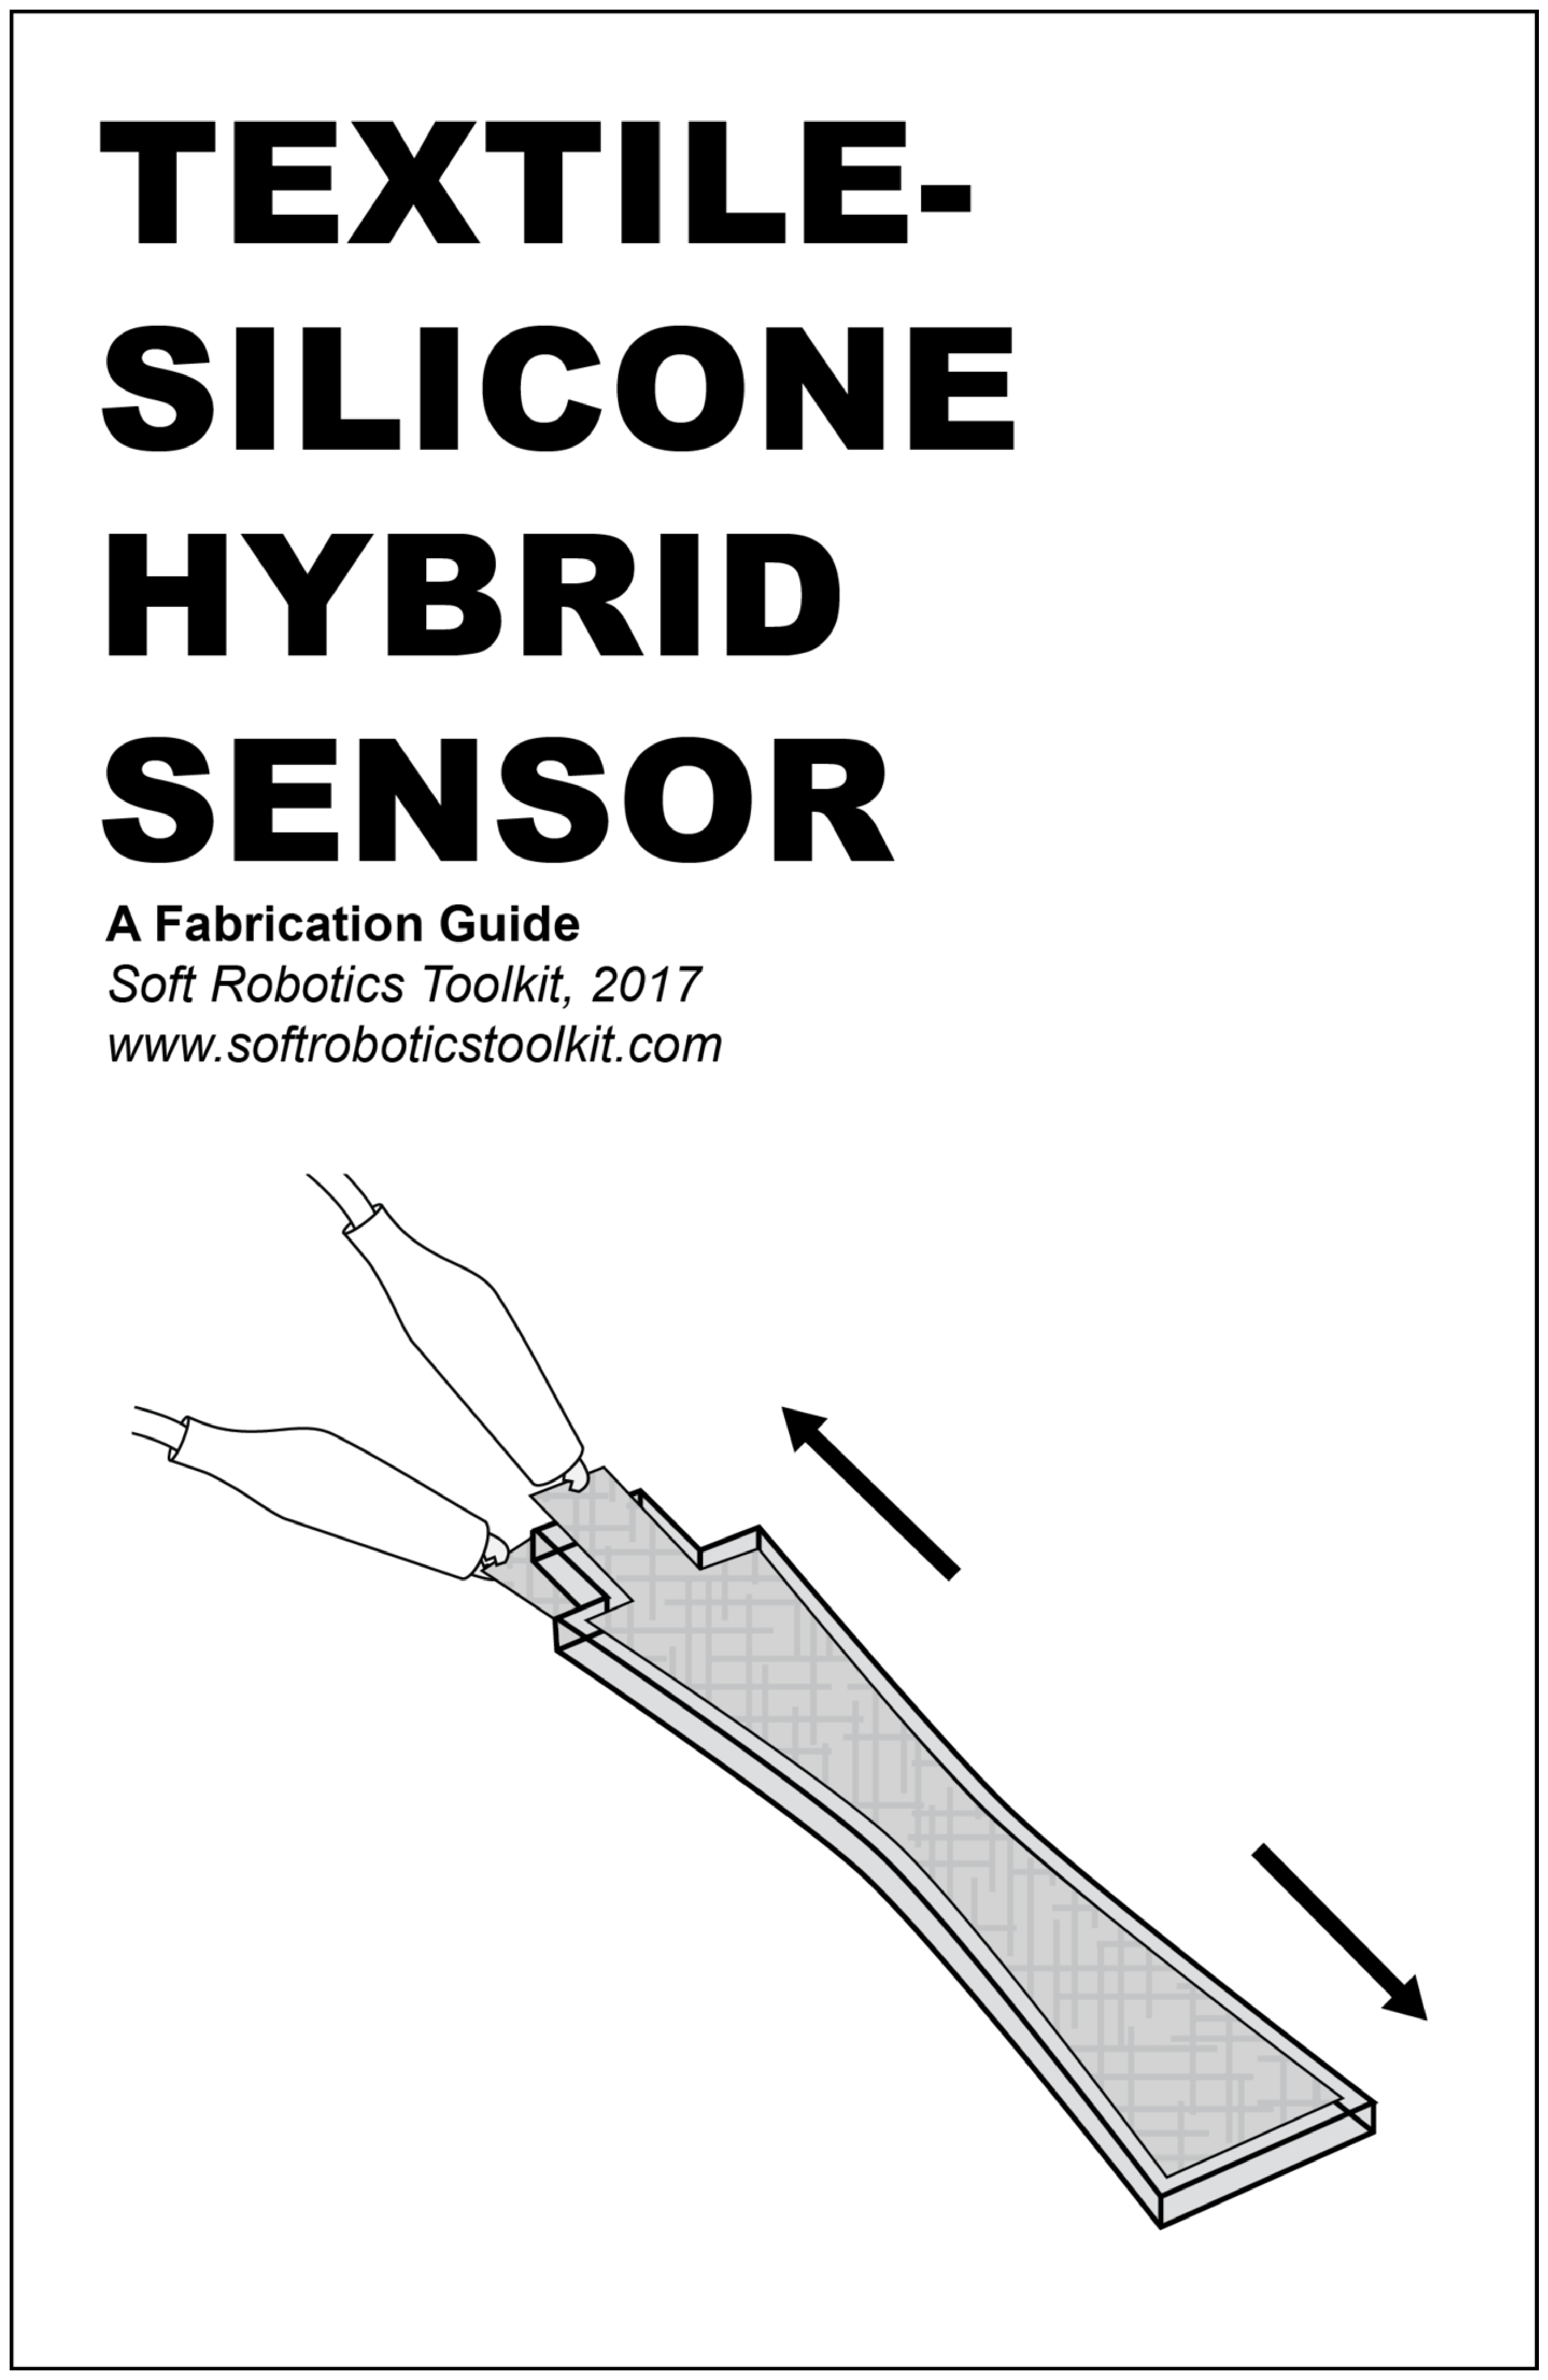
\includegraphics[width=0.5\columnwidth]{./1_prolusion/MITSoftRobotics.eps}
        \caption{ストレッチセンサ模式図\cite{MITSoftRobot}}
        \label{MITSoftRobot表紙}
    \end{center}
\end{figure}

\subsection{ペダリングロボット}
先行研究として,人間の筋肉を模した空気圧人工筋をもちいたペダリングロボットが存在する.
これは,人間のペダリング動作における筋シナジーの計測を行い,ロボットに再現させるものであった.
筋シナジーの計測は片麻痺患者,健常者ともに行い,片麻痺患者におけるペダリング動作時の特徴的な
活動状態を健常者との比較で行った.ヒトの運動解析を行い,運動戦略を明らかにするために製作され
使用されたロボットである.本ロボットは,腰がサドル上に固定された状態で股関節,膝関節,足関節
それぞれがピッチ方向にのみ自由度を持っており2次元平面上における動作を再現することが出来た.
これらの動作を再現するために,空気圧人工筋がヒラメ筋,前脛骨筋,大腿四頭筋,大腿二頭筋,腸腰筋,恥骨筋の
6筋分が搭載された形となっている.なお,空気圧人工筋の出力上,日本人成人男性の半分の重量モデルで作製さている.\cite{watanabe}
\begin{figure}[h]
 \begin{center}
  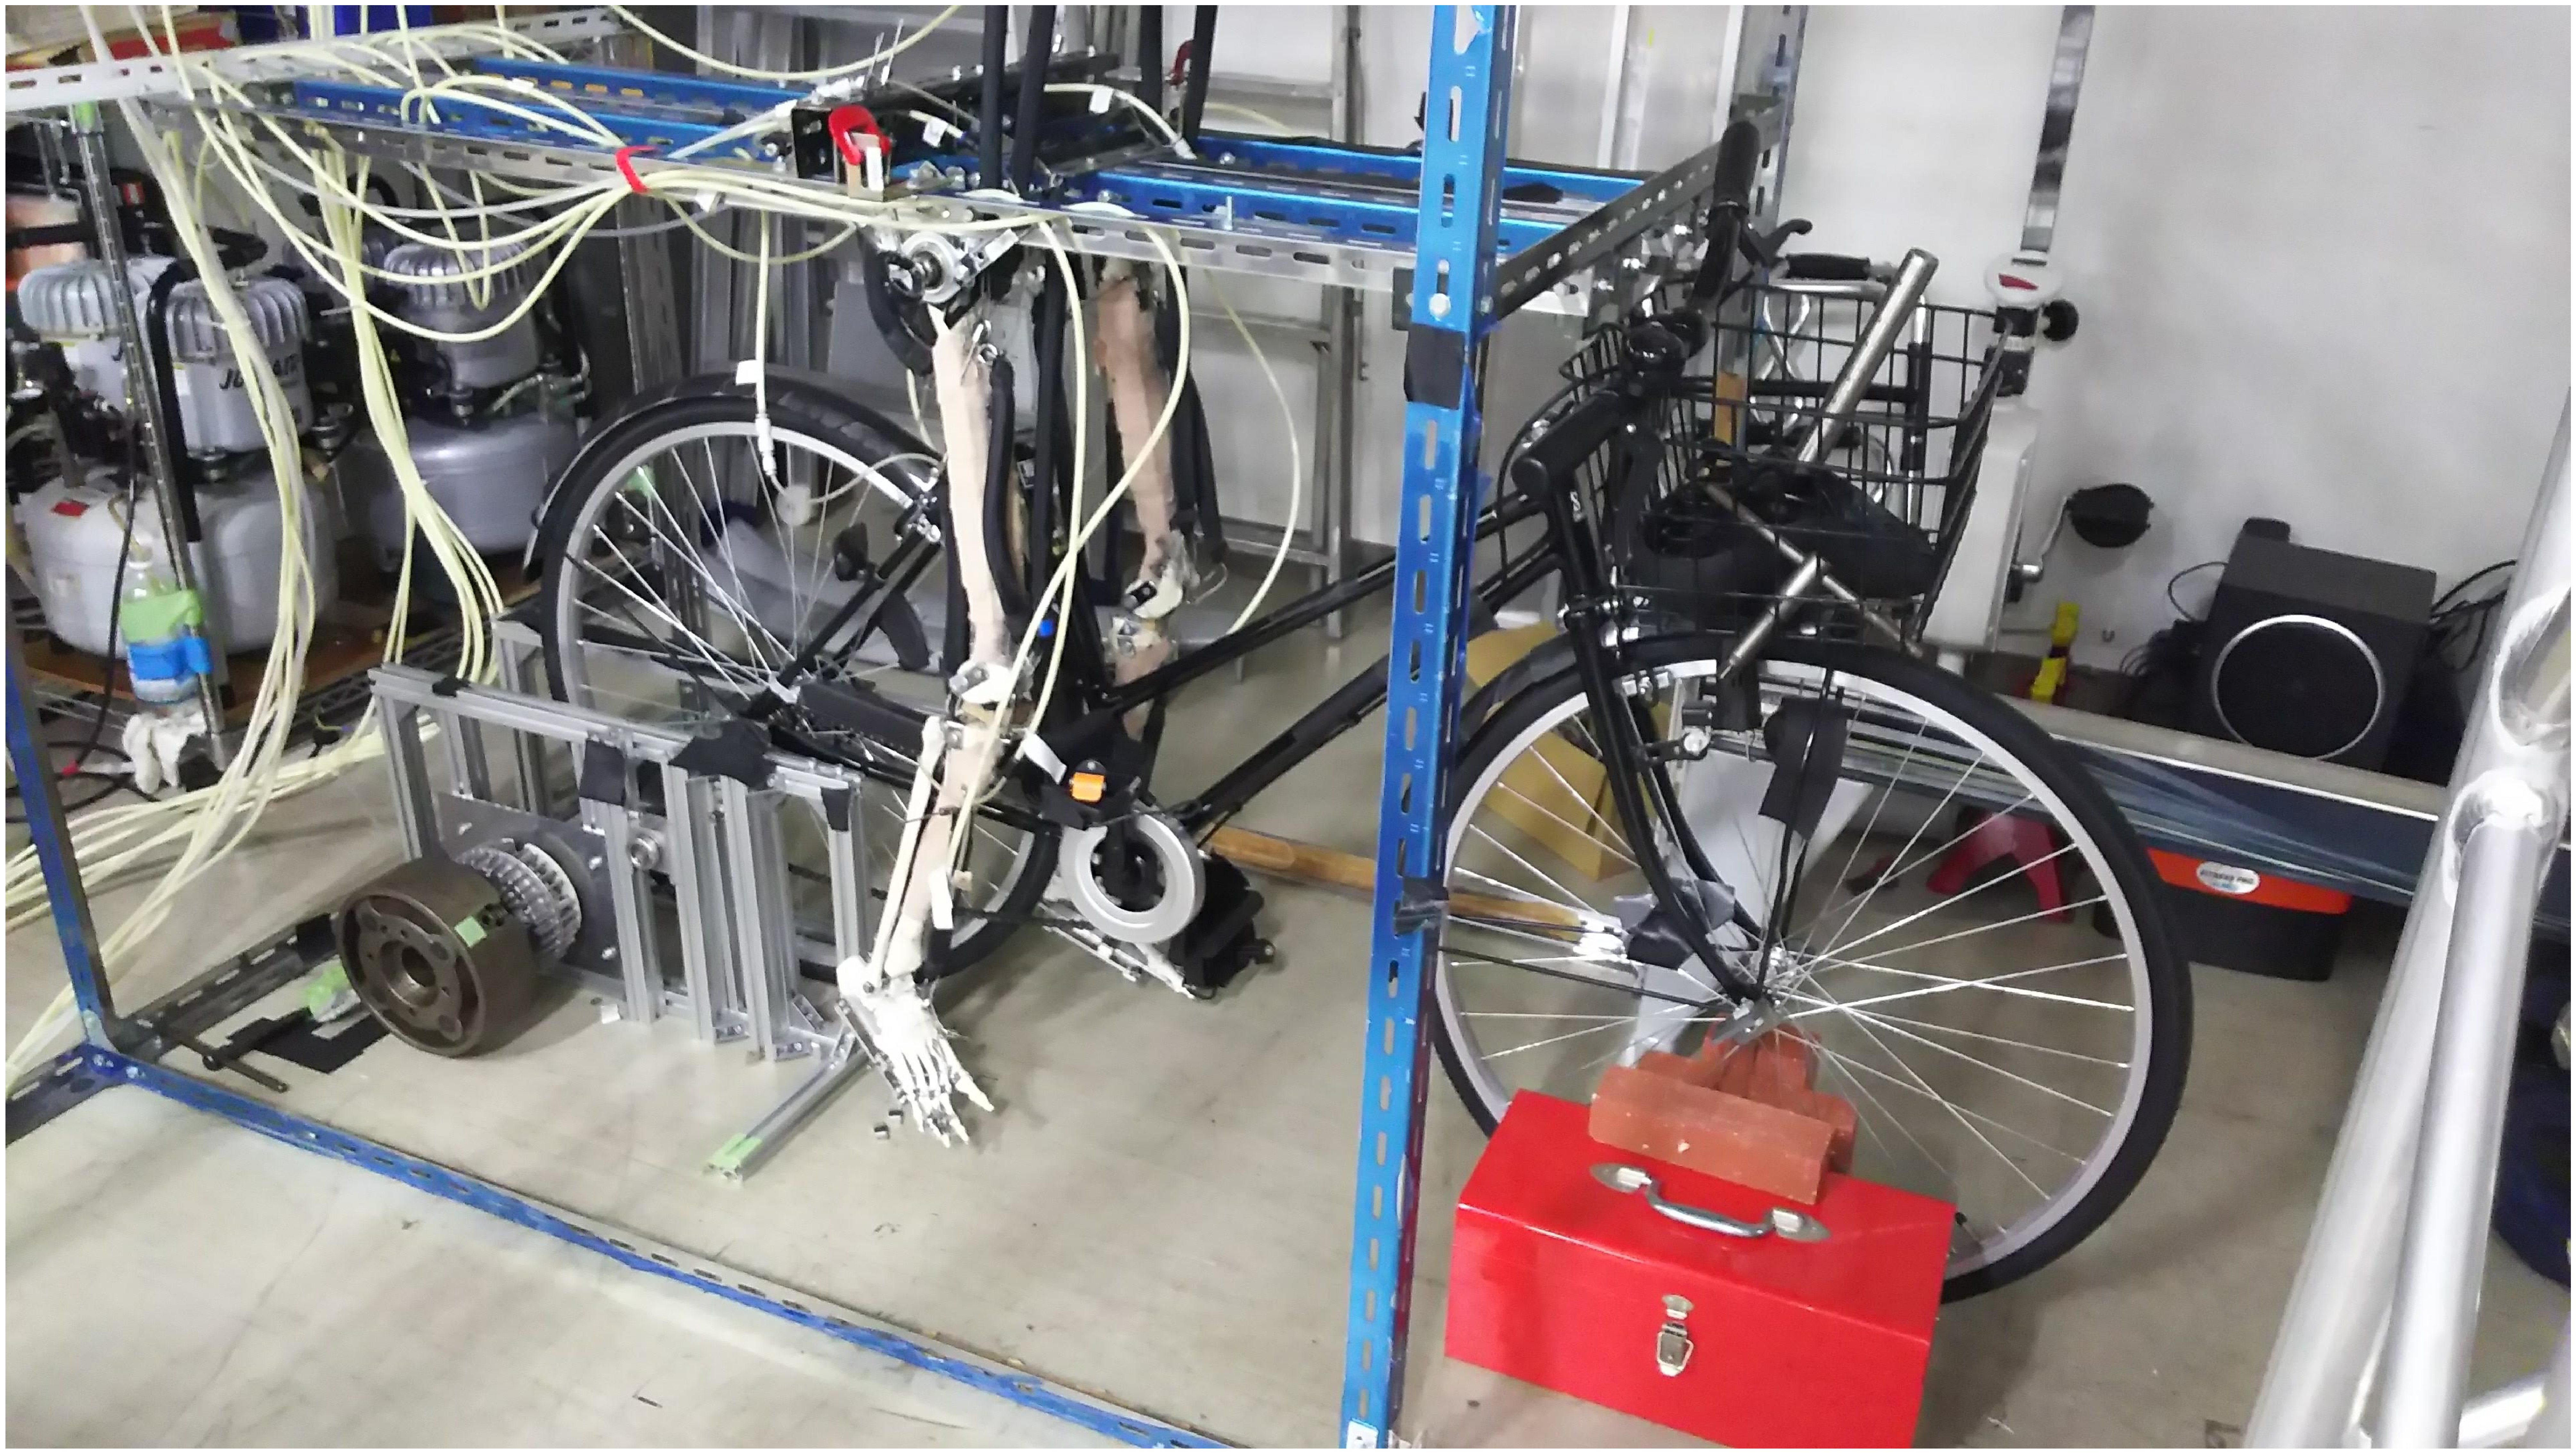
\includegraphics[width=0.75\columnwidth,clip]{./1_prolusion/1st.eps}
  \caption{ペダリングロボット}
  \label{初号機}
  \end{center}
\end{figure}

\newpage

\subsection{二足歩行ロボット}
%TODO:2号機のお話を書く
%TODO:2号機関連の研究のリファレンスを貼る
先述のペダリングロボットの研究成果を生かし,腰椎を固定していない状態の二足歩行ロボットが製作された.
本ロボットは,腰椎が固定されていないことにより立脚時の歩容動作の再現を行えるようになった.
なお,動作時は自重を支えることができないため,股間部の支持を行った.また,関節動作に関しては
先述のロボットと同様の形となっており,股関節,膝関節,足首関節それぞれがピッチ方向にのみ自由度を持っており
2次元平面上における動作を再現することが出来た.これらの動作の再現を行うため,空気圧人工筋が
ヒラメ筋,前脛骨筋,大腿四頭筋,大腿二頭筋,腸腰筋,恥骨筋の6筋分が搭載された形となっている.

これらの研究によって平衡点仮説に基づく筋シナジー解析を用いた歩行動作の解明の為に用いられた.
この歩行動作解析により,健常者の歩行と片麻痺患者の歩行の動作の相違に関して解明することができた.
\begin{figure}[h]
  \begin{center}
  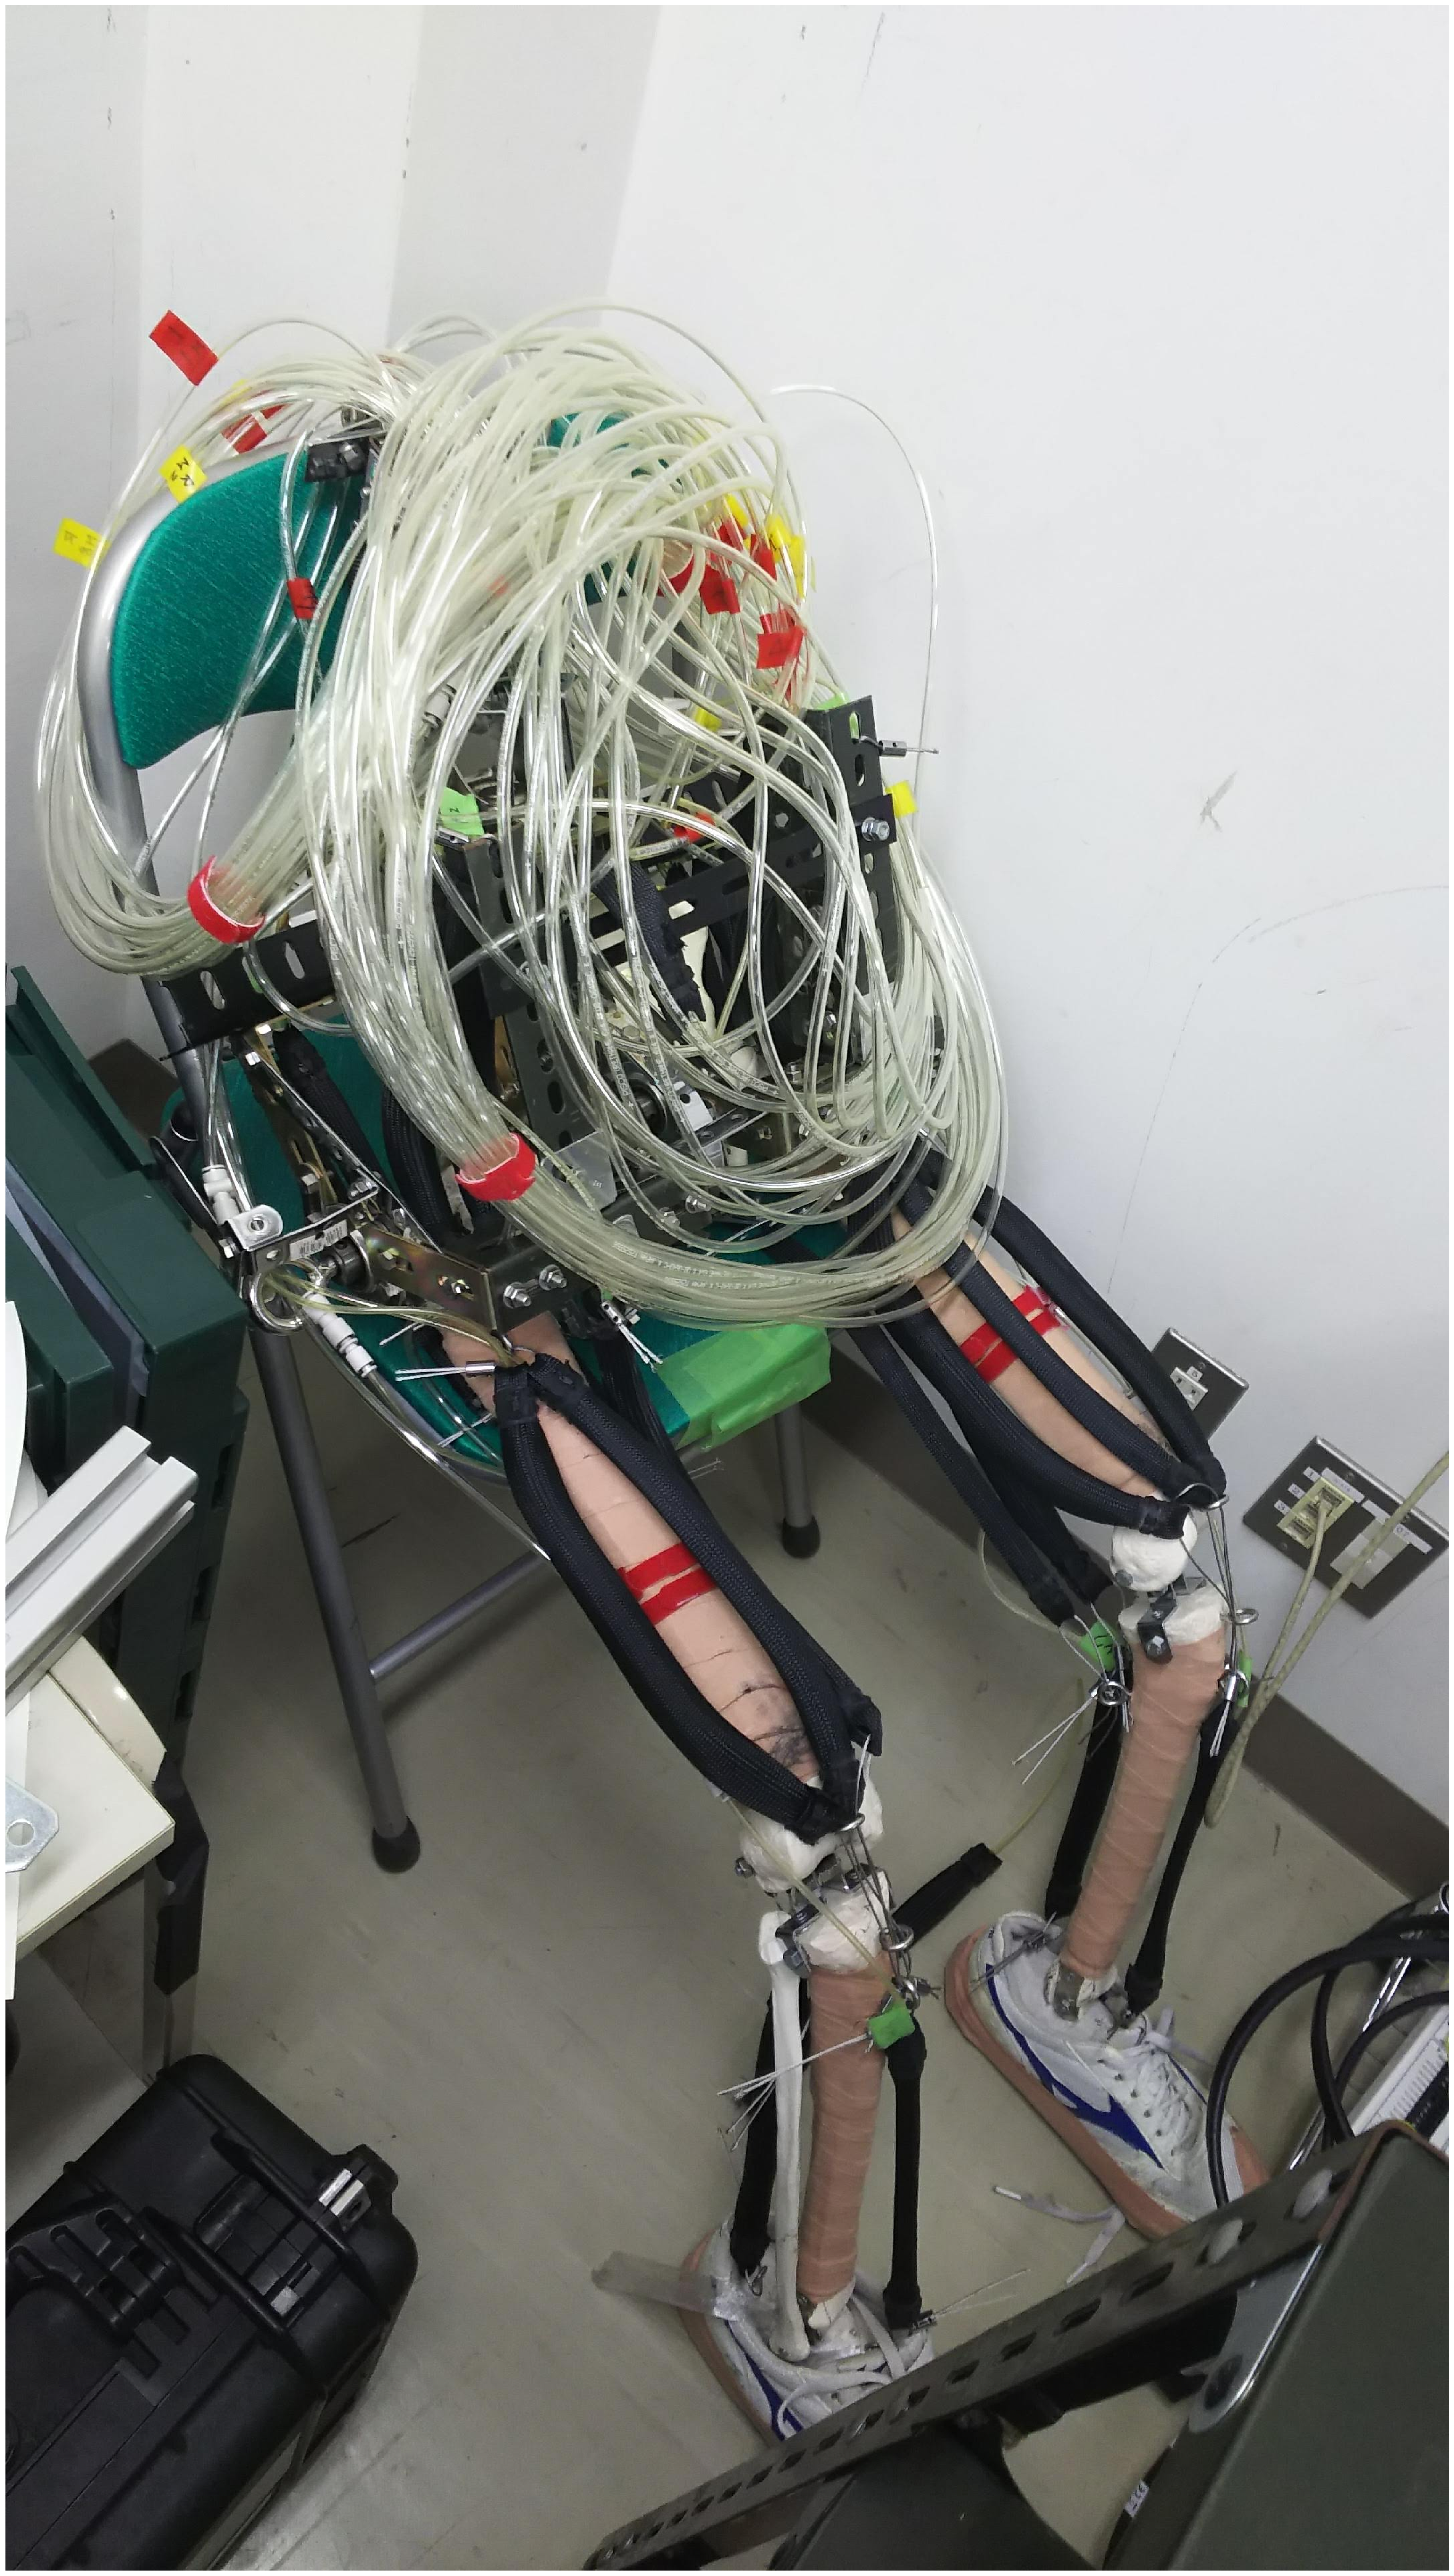
\includegraphics[width=0.35\columnwidth,clip]{./1_prolusion/2nd.eps}
  \caption{二足歩行ロボット}
  \label{2号機}
 \end{center}
\end{figure}

\newpage

\section{研究目的}
%TODO:これらを統合し,筋肉の伸長を巻き込んだシステムの話をする
先述の先行研究例を踏まえ,やわらかいアクチュエータである空気圧人工筋の伸長計測をフレキシブルストレッチセンサを用いて計測を
行うことを一つの目的とする.そのために,導電性布を用いたフレキシブルストレッチセンサの製作を行った.また,センサ自体を自作するため,
本センサの計測系の設計製作も行った.

また,ペダリングロボット,2足歩行ロボットの経験を踏まえ,新たに足関節ロボットの製作を行った.
これは,従来のロボットでは足関節部分の自由度がピッチ方向のみの1自由度であり,動作空間が2次元平面のみに制限されていた.
一方で実際の人間の自由度はこれに加えてロール方向,ヨー方向も存在し3自由度である.
3自由度にすることで平面動作だけでなく空間的な動きも可能になる.
加えて自由度の増加により,前後方向の移動だけでなく,横方向への移動も可能となり人間動作の再現性が向上するとも考えられる.

最終的に,導電性布を用いたストレッチセンサと新たに製作した足関節ロボットを用いて,人間の筋の伸長を計測することを,研究の最終目的とする.

\section{論文構成}
本論文の構成は以下の通りである.
{\bf 第2章}で動作モデルと足関節ロボット,ストレッチセンサの製作過程について述べ,{\bf 第3章}で計測アルゴリズムと実験手法に関して示す.
{\bf 第4章}では結果を示し、ストレッチセンサの性能評価に関して考察する.
最後に{\bf 第5章}で本論文の成果をまとめる.

\chapter{動作モデル・実験器具製作}
\section{動作モデル}
\subsection{ストレッチセンサ}
伸縮センサはFig.\ref{fig:伸縮センサ全体図},Fig.\ref{fig:伸縮センサ断面図}において示す通り,
柔軟で弾性変形する伸縮性シリコン(絶縁層)と導電性布電極(導電層)の重ね合わせによって構成されている.
これは,誘電体をシリコン,極板を導電性布としたコンデンサとなっている.

\begin{figure}[h]
    \begin{center}
        \label{fig:伸縮センサ全体図}
        \includegraphics[width=0.5\columnwidth,clip]{./2_measurement/slide1.eps}
        \caption{伸縮センサ全体図}
    \end{center}
\end{figure}
\begin{figure}[h]
    \begin{center}       
        \label{fig:伸縮センサ断面図}
        \includegraphics[width=0.5\columnwidth,clip]{./2_measurement/slide2.eps}
        \caption{伸縮センサ断面図}
    \end{center}
\end{figure}

ここで伸縮センサ中の導電性布の長さ$l$、幅$w$,シリコンの厚さを$d$,シリコンの誘電率を$\epsilon{}_s$とすると,
\begin{eqnarray}
    C=\epsilon{}_s\frac{lw}{d}
    \label{eq:cap}
\end{eqnarray}
といった式でその静電容量$C$が求められる.

伸縮センサに引張方向に力を加えると、センサーの長さが増加する。また、それに伴って、厚み、幅も変化する。
ここで変化により、導電性布の長さが$\Delta{l}$、幅が$\Delta{w}$、シリコンの厚みが$\Delta{d}$変化したとすると、先ほどの式\ref{eq:cap}より、静電容量の変化量$\Delta{C}$は、
\begin{eqnarray}
    C+\Delta{C} &=& \epsilon{}_s\frac{(l+\Delta{l})(w+\Delta{w})}{(d+\Delta{}d)}\\
    & \simeq & \epsilon{}_s\frac{lw+l\Delta{w}+w\Delta{l}}{d+\Delta{d}}\\
    &=&\frac{Cd}{lw}\left(\frac{lw+l\Delta{w}+w\Delta{l}}{d+\Delta{d}}\right)\\
    (C+\Delta{C})(d+\Delta{d})&=&Cd\left(1+\frac{\Delta{w}}{w}+\frac{\Delta{l}}{l}\right)\\
    Cd+C\Delta{d}+d\Delta{C}& \simeq &Cd\left(1+\frac{\Delta{w}}{w}+\frac{\Delta{l}}{l}\right)\\
    \Delta{C}&=&Cd\left(\frac{\Delta{w}}{w}+\frac{\Delta{l}}{l}-\frac{\Delta{d}}{d}\right)
    \label{eq:deltaC}
\end{eqnarray}
といった式で示される.ここで、長さ方向の工学ひずみを$\epsilon_l$、幅方向の工学ひずみを$\epsilon_w$、厚み方向の工学ひずみを$\epsilon_d$とそれぞれすると、式\ref{eq:deltaC}は、
\begin{eqnarray}
    \Delta{C}=Cd(\epsilon_w+\epsilon_l-\epsilon_d)
    \label{eq:epsilonC}
\end{eqnarray}
といった式で表すことができる.幅、厚み方向のポアソン比を$\nu_w$、$\nu_d$とすると、式\ref{eq:epsilonC}より、
\begin{eqnarray}
    \Delta{C}=Cd\epsilon_l(1+\nu_w-\nu_d)
\end{eqnarray}
となる。ゆえに、長さ$l$が変化すると、静電容量$C$が変化することが示される。今回は、このことを利用しストレッチセンサーの長さの変化を静電容量の変化として計測を行った。

\subsection{フレキシブルストレッチセンサ計測回路}\label{sec:RC回路}
%TODO:伸縮センサ計測回路に関しての記述を行う
先述の通り,伸縮センサは静電容量の変化で伸縮状況を示す.故に今回は静電容量の変化を計測することができる回路の製作を行った.
静電容量の計測を行う方法として、LRCメータやインピーダンスアナライザを用いる方法が挙げられる。
これらの計測機器を用いると静電容量の変化を高精度に計測することができる。しかし、1ch当たりの
計測機器の単価が非常に高く、また既存のフィードバック系に組み込みにくいといった状況があった。そこで、
今回はより安価で手軽な方法である、RC回路を用いた方法をとった。

下記のFig.\ref{fig:RC}に示したRC回路を用い、Vinに入力を与えるとVoutで信号が立ち上がるまでに
時間の遅れが発生する。これは、抵抗値$R$、静電容量$C$とすると、時定数$\delta t$は、
\begin{eqnarray}
    \delta t = RC
\end{eqnarray}
といった式であらわされる。なお、この遅れ系の現象を計測すると、Fig.\ref{fig:出力状態図}の様になる。

\begin{figure}[h]
 \begin{center}
    %TODO:Voutの向きを出力にする
  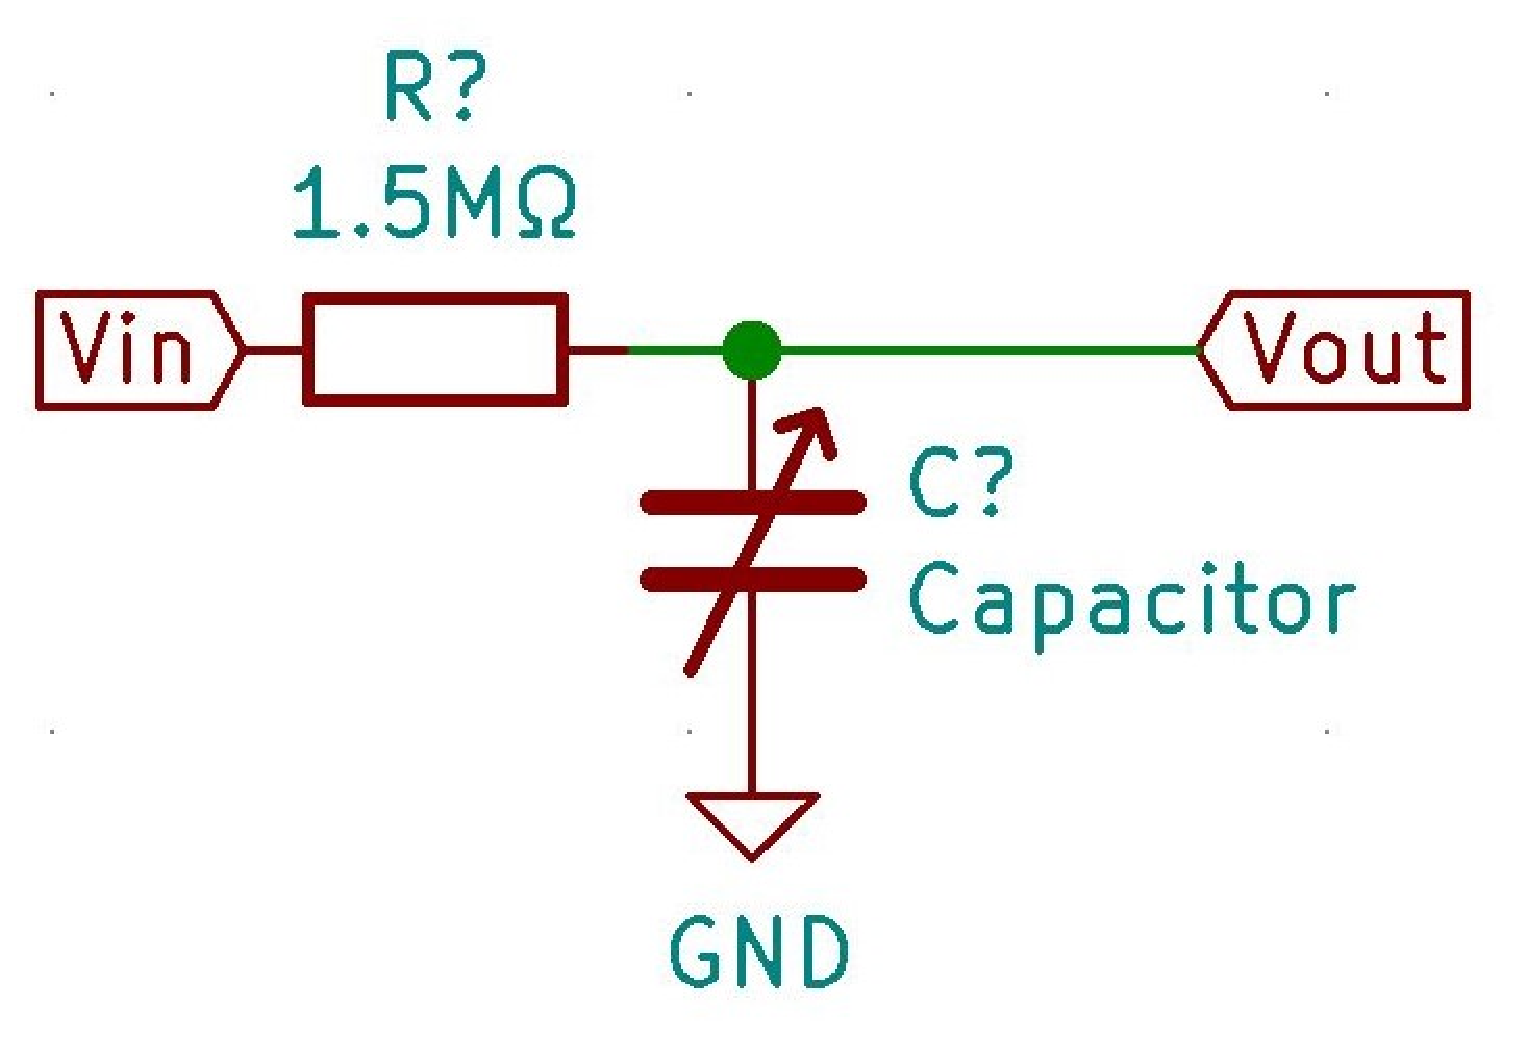
\includegraphics[width=0.5\columnwidth,clip]{./2_measurement/RC.eps}
  \caption{RC回路}
  \label{fig:RC}
 \end{center}
\end{figure}

\begin{figure}[h]
    \begin{center}
     \includegraphics[width=0.5\columnwidth,clip]{./2_measurement/oscilloscope.eps}
     \caption{fig:出力状態図}
     \label{オシロスコープ}
    \end{center}
\end{figure}

これらの計測に関して,1つのマイコンを用いて複数の伸縮センサの計測を行うと計測周期が低下し,
計測精度の低下が懸念された.これを踏まえ,1つのマイコンで計測を行う伸縮センサの数を2個とした.
一方で今回,足首を中心とした筋の伸縮の計測を行うため3チャンネル分の計測を行う必要がある.
故に,マイコン3枚分の計測システムを用意した.同期信号を用いて計測のデータ取得,同期を行った.
\begin{figure}[h]
 \begin{center}
  \includegraphics[width=0.5\columnwidth,clip]{./2_measurement/circuit.eps}
  \caption{計測時に実際に用いた基板}
  \label{fig:circuit}
 \end{center}
\end{figure}

\newpage

\subsection{足関節における筋肉}
%TODO:足首周りの動作関係のお話をする
%TODO:筋肉のお話もする
Fig.\ref{fig:legMuscle}において、脚部における筋肉状況を示す。これらの脚部筋肉のうち足関節の動作に
寄与している物はヒラメ筋、長腓骨筋、前脛骨筋、長母趾伸筋、長趾伸筋といったものが挙げられる。

従来のペダリングロボット、2足歩行ロボットの足関節部分では前脛骨筋、ヒラメ筋のみに注目し
それらの筋肉の再現を、空気圧人工筋を用いて行った。
今回製作する足関節ロボットでは実際の人間の動作の再現を行うため、従来のピッチ方向のみの動作を
想定した設計では目的を満たすことができない。そこで、従来注目していた、前脛骨筋、ヒラメ筋に
加えて、長腓骨筋も注目するようにした。また、従来のロボットでは足関節部分はピンジョイントを用いて、
動作方向の制限を行っていたが、今回はボールジョイントを用い、動作方向の制限をなくし、ロール・ピッチ・ヨー各方向に
自由度を持たせることができた。
\begin{figure}[h]
    \begin{center}
     \includegraphics[width=0.5\columnwidth,clip]{./2_measurement/legMuscle.eps}
     \caption{脚部における筋肉状況}
     \label{fig:legMuscle}
    \end{center}
\end{figure}

\newpage

\section{実験器具の製作}
\subsection{伸縮センサ製作}
\begin{enumerate}
    \item 3Dプリンターを用いて伸縮センサのサイズに合った型を用意する.
    \item 導電性布を型に合わせて鋏を用いて切る.
    \item 導電性布に錫めっき線を縫い通し,型の上に導電性布を置く.この際,錫めっき線が型の外に出てくるようにする.
    \item 上から硬化剤を混ぜたシリコン流し込み固まるまで数時間放置.
    \item シリコンが固まったら2枚目の導電性布に1枚目と同様に錫めっき線を通し硬化したシリコンの上に置く.
    \item その上から硬化剤を混ぜたシリコンを薄く塗り固まるまで放置.
    \item 最後のシリコンが硬化したら型から取り外し,錫めっき線に銅線接続し,コネクタをつけて完成.
\end{enumerate}
\subsection{足関節ロボット製作}

先述のとおり、以前製作されたペダリングロボット、2足歩行ロボットの経験をもとに足関節ロボットの製作を行った。
以下に足関節ロボットの製作過程を示す。
%TODO:使用した人体模型の種類の記述を行う。

今回、足関節ロボットの骨格としてFig.\ref{fig:bodyBone}人体模型を用いた。本模型から必要となる、膝より下の部分を取り外した。
取り外した結果、Fig.\ref{fig:legBone}の様になった。
\begin{figure}[h]
    \begin{center}
     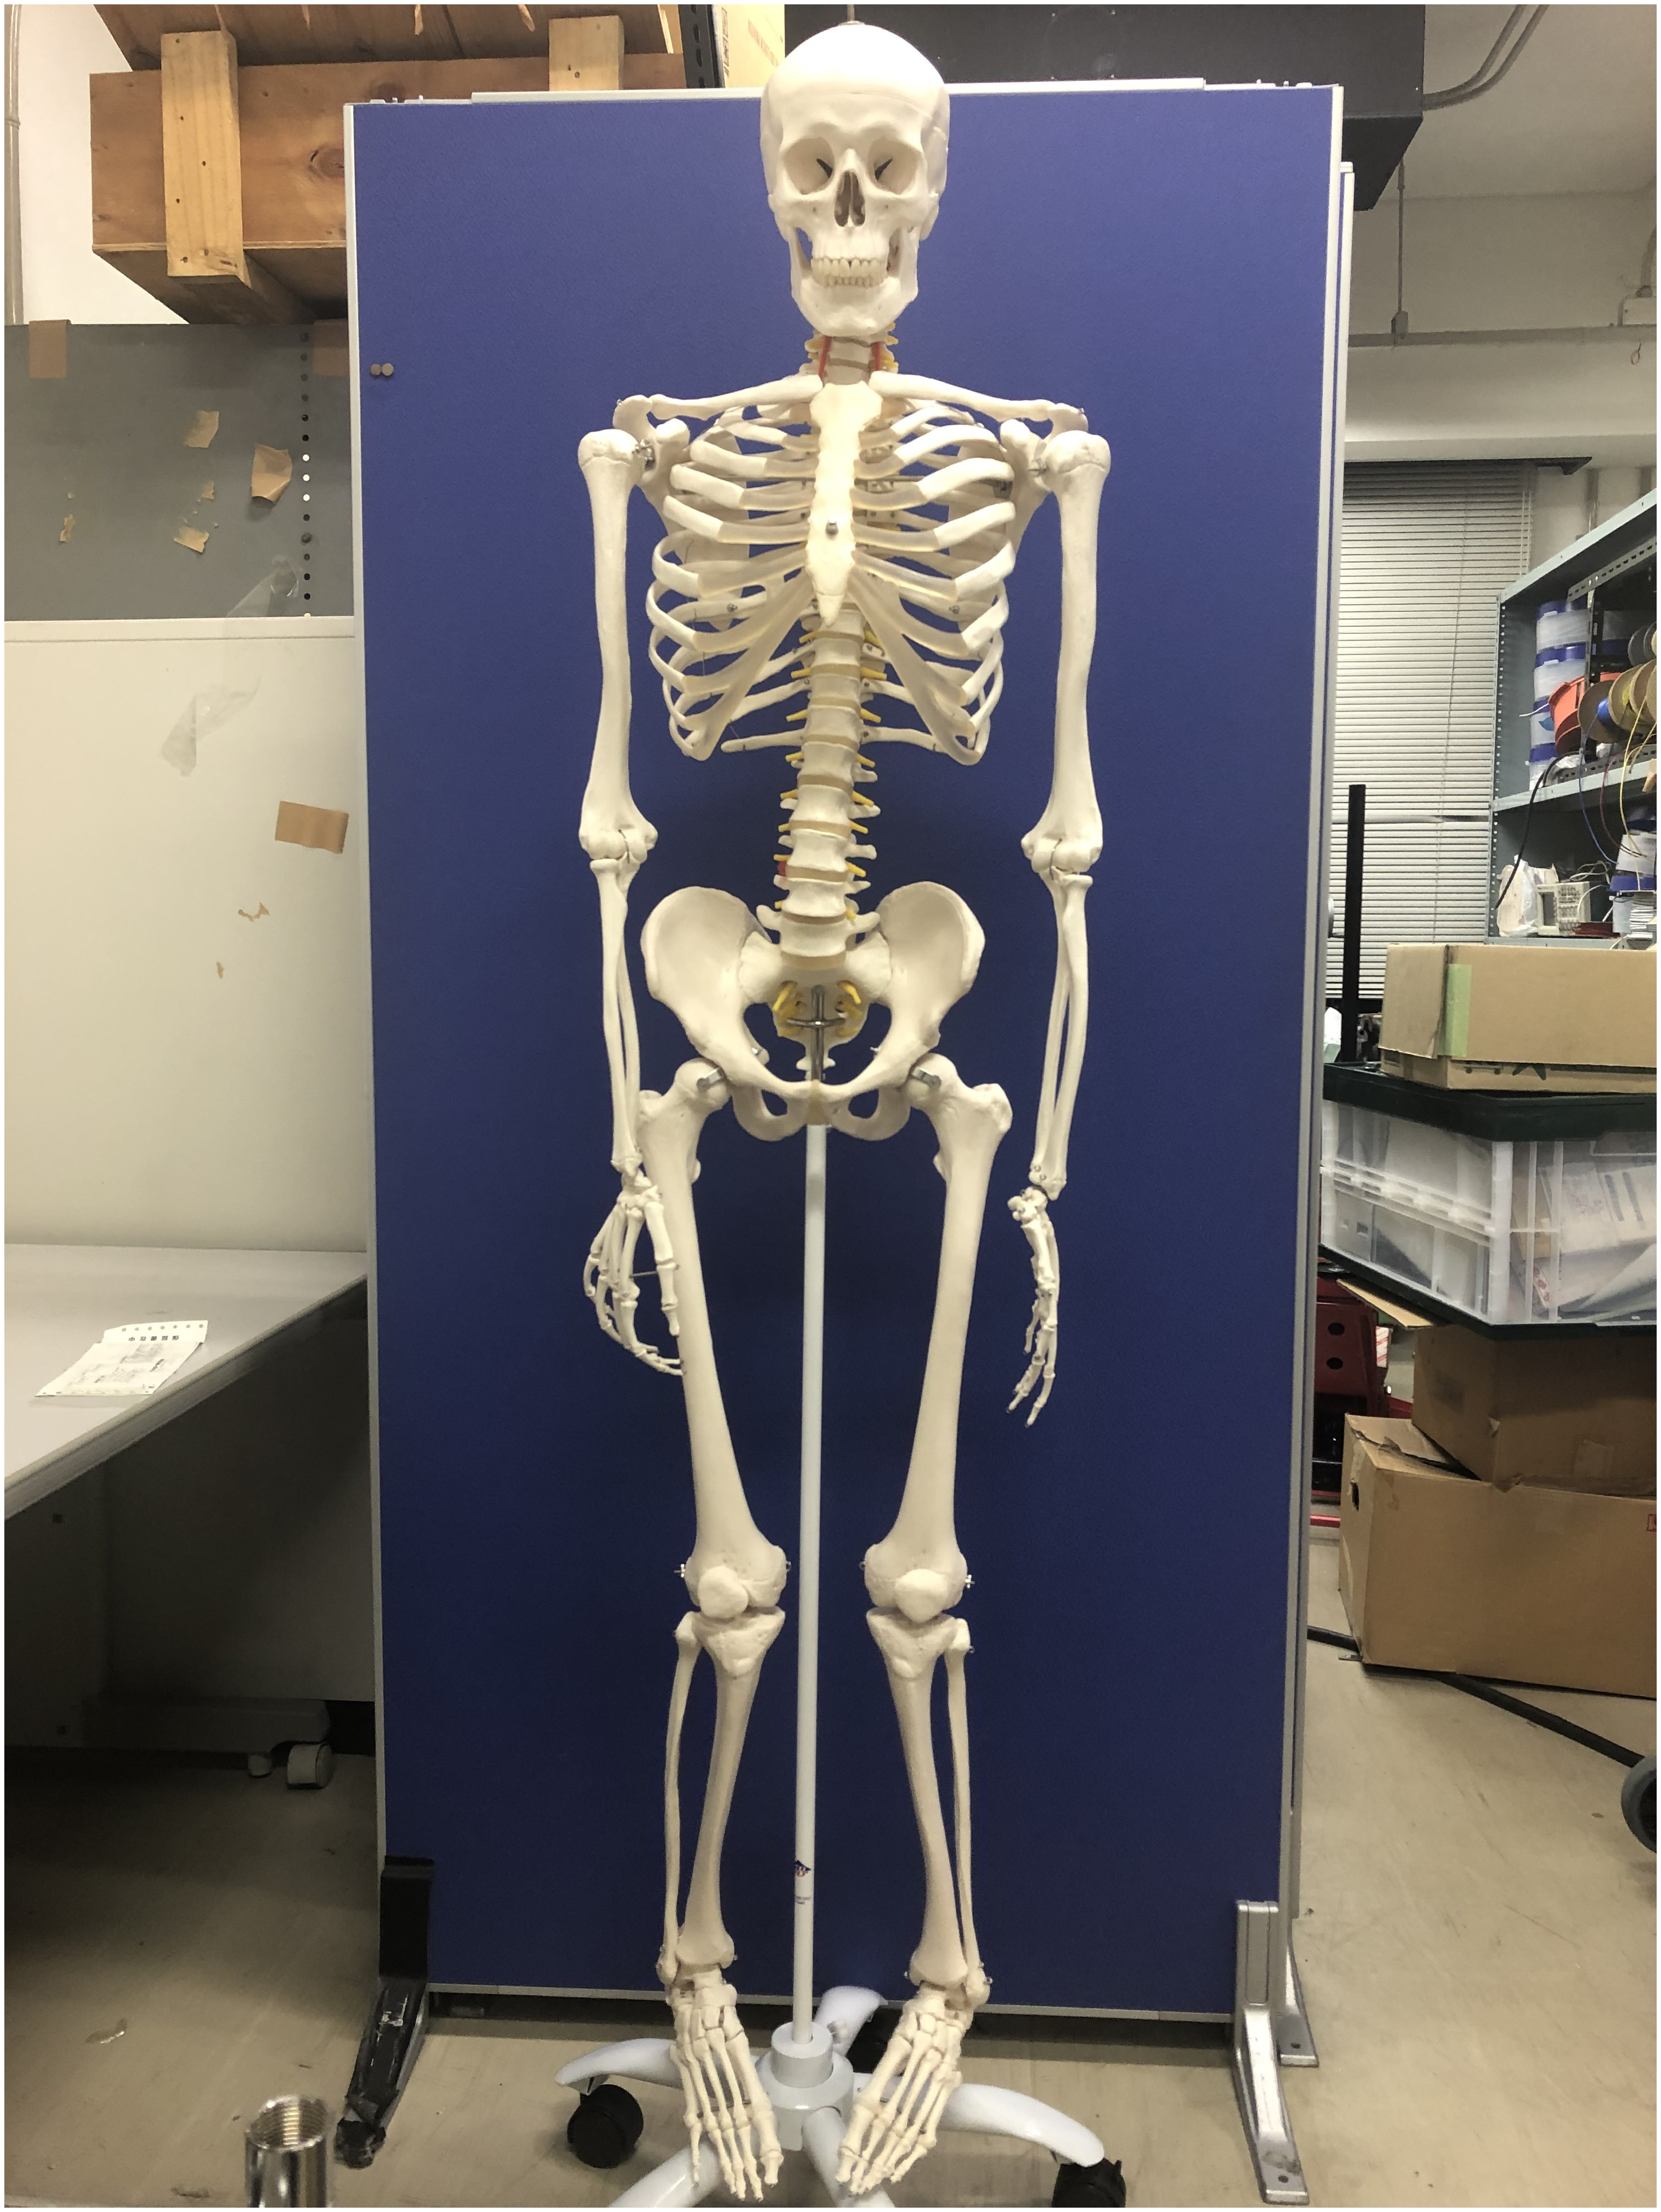
\includegraphics[width=0.4\columnwidth,clip]{./2_measurement/bodyBone.eps}
     \caption{人体模型骨格(全身)}
     \label{fig:bodyBone}
    \end{center}
    \begin{center}
     \includegraphics[width=0.6\columnwidth,clip]{./2_measurement/legBone.eps}
     \caption{人体模型骨格(脚部)}
     \label{fig:legBone}
    \end{center}
\end{figure}
\newpage
以前製作されたペダリングロボット、2足歩行ロボットでは関節部分にピンジョイントを用いていたが、今回製作する足関節ロボットでは、
自由度を向上させることを一つの目的としているので、膝部分にピンジョイント、足首部分にボールジョイントを用いた。

まず初めに前脛骨筋の両端を彫刻刀やバンドソーを用いて平面を作成した。続いてそこに、ボルト/ナットを用いてボールジョイント、ピンジョイントの軸受けの
固定を行った。そして、人間の筋付着位置に合わせて空気圧人工筋を接続するため、リングボルトを設置した。その結果、下記のFig.\ref{fig:legJoint}の様になった。

\begin{figure}[h]
    \begin{center}
     \includegraphics[width=0.6\columnwidth,clip]{./2_measurement/legJoint.eps}
     \caption{ジョイント、リングボルト接地状態(脚部)}
     \label{fig:legJoint}
    \end{center}
\end{figure}
次に重心位置を人間のものと合わせ、重量を成人男性の1/2にする作業を行った。
人体模型の骨は樹脂でできているため軽量であるので、鉛シートを巻き調整を行った。
重心位置の確認には紐で巻いて垂らし、その鉛直線が交わるところで求めた。
重量、重心位置の調整を行った結果、Fig.\ref{fig:legPb}の様になった。

\begin{figure}[h]
    \begin{center}
     \includegraphics[width=0.6\columnwidth,clip]{./2_measurement/legPb.eps}
     \caption{鉛シートを巻いた結果}
     \label{fig:legPb}
    \end{center}
\end{figure}
\newpage
続いて、足の製作を行った。前脛骨筋と同様に、人間の筋付着位置に合わせて空気圧人工筋の
接続をするリングボルトの設置をした。また、補強用として足の裏部分にアルミ板を固定した。
そして、ボールジョイント接続部分に穴をあけタップドリルを用いてねじ溝を掘った。

\begin{figure}[h]
    \begin{center}
     \includegraphics[width=0.6\columnwidth,clip]{./2_measurement/foot.eps}
     \caption{リングボルト設置結果(足上面)}
     \label{fig:foot}
    \end{center}
    \begin{center}
     \includegraphics[width=0.6\columnwidth,clip]{./2_measurement/footside.eps}
     \caption{リングボルト設置結果(足側面)}
     \label{fig:footside}
    \end{center}
\end{figure}

その後、指先と踵の間を丁番を用いて接続し、ピッチ方向に自由度を持たせた。
なお、空気圧人工筋などの能動的なアクチュエータは用いず、接地時に可動する受動的なものとして用いる様にした。
そして、その足にシリコン材を用いて肉付けを行い、重量、重心位置の調整をおこなった。
この時、脛骨と同様に重心位置は成人男性、重量は成人男性の1/2となるように調整をおこなった。
なお、脛骨と異なり鉛シートを用いずシリコン材を用いたのは衝撃吸収と成型性のしやすさからその様にした。
\newpage
\begin{figure}[h]
    \begin{center}
     \includegraphics[width=0.6\columnwidth,clip]{./2_measurement/siliconfoot.eps}
     \caption{シリコン材,丁番設置結果(足上面)}
     \label{fig:foot2}
    \end{center}
    \begin{center}
     \includegraphics[width=0.6\columnwidth,clip]{./2_measurement/siliconfootside.eps}
     \caption{シリコン材,丁番設置結果(足側面)}
     \label{fig:footside2}
    \end{center}
\end{figure}

続いて、脛骨と足部をボールジョイントのねじを用いて接続した。そして、人間の前脛骨筋、長腓骨筋、ヒラメ筋にあたる
空気圧人工筋3本を、それぞれワイヤーを用いてリングボルトと接続した。最後に、足部に靴を履かせて完成した。
完成したものは、Fig.\ref{fig:legPb}である。

\begin{figure}[h]
    \begin{center}
     \includegraphics[width=0.75\columnwidth,clip]{./2_measurement/fin.eps}
     \caption{完成した足関節ロボット}
     \label{fig:legPb}
    \end{center}
\end{figure}
\chapter{計測・実験手法}
\section{伸縮センサ計測アルゴリズム}
\section{伸縮センサ計測データ処理}
\chapter{結果・考察}
\section{床反力}
フォースプレートにより得られた鉛直方向の床反力データ{\bf Fig. \ref{force}}を用いて周期の切り出しを行う.接地時から次の接地時までを1周期とする.そして接地時から離地時までを立脚期,離地時から接地時までを遊脚期とする.
 
 また,被験者A,Bの1周期における立脚期の割合を{\bf Table }\ref{stance}に示す.このデータによると,AはBに比べ立脚期の割合が大きいことがわかる.
 
\begin{table}[!h]
 \caption{Ratio of Stance.}
 \begin{center}
  \begin{tabular}{|c|c|c|} \hline
    & Subject A & Subject B \\ \hline \hline
  Stance Ratio[%] & 0.616885 & 0.576601 \\ \hline
  \end{tabular}
  \label{stance}
 \end{center}
\end{table}

さらに床反力データを1周期で平均化し({\bf Fig. \ref{FR}}),そのデータから鉛直方向への力積を導出した.そして力積をそれぞれの被験者の体重で除することで,立脚期の速度変化量を導出した{\bf Table }\ref{ISV}.
 
 \begin{table}[!h]
 \caption{Impluse and speed Variation.}
 \begin{center}
  \begin{tabular}{|c|c|c|} \hline
    & Subject A & Subject B \\ \hline \hline
   Impulse[$kg*m/s$] & 783.038 & 899.41 \\ \hline
  Speed Variation[$m/s^2$] & 13.0506 & 14.2763 \\ \hline
  \end{tabular}
  \label{ISV}
 \end{center}
\end{table}

{\bf Table }\ref{ISV}より,被験者Aに比べ被験者Bの方が大きな加速度を得ているため,より高く跳躍していると示される.よって,鉛直方向への跳躍は被験者Bが優れているといえる.

\newpage
\section{運動学データ}
OptiTrackより所得した運動学データを解析し,被験者A,Bの鉛直方向の重心位置の遷移と,各関節角度の遷移を{\bf Fig. \ref{gp}},{\bf Fig. \ref{angle}}に示す.重心位置は簡易化のために両腰関節の中点としている.
 
 重心位置の遷移を見ると,被験者A,B共に同様の軌跡をとっている.離地時の重心位置は被験者Aの$0.647816$,被験者Bの$0.598195$に対し,最高到達点は被験者A$0.913786$,被験者B$0.904918$となっている.この点からも,被験者Bは被験者Aよりも15%高く跳躍していることがわかる.
 また角度に関しては,傾きの大きさこそ違うが,被験者A,B共に相似している.
 
 \newpage

\section{%MVC,筋拮抗和,筋拮抗比}
本実験より,被験者A,Bの右脚から得られた主要8筋($m_1$~$m_8$)の%MVC,4対の筋拮抗和($s_1$~$s_4$),筋拮抗比($r_1$~$r_4$)の時間変化の様子を{\bf Fig. \ref{m14}}~{\bf Fig. \ref{r14}}に示す.
 
\newpage 
各筋のEMGデータを比較すると,被験者AとBで1周期における筋の活動が大きく異なっている.$m_2$,$m_8$は被験者A,B共に似通った筋活動をしているが,$m_1$,$m_4$,$m_5$は被験者Bに対して被験者Aは着地時に強く筋を緊張させている.
 筋拮抗和にも着目すると,接地時に被験者Aは筋拮抗和を高めているのに対し,被験者Bは高めていない.
これは着地時の衝撃吸収における運動戦略の違いであると考えられる.被験者Aは走行時と同様に各関節の剛性を高めることで次の運動に繋げようとしているのに対し,被験者Bは剛性を落とすことによる着地時の衝撃吸収を目的としていると考えられる.
一方,被験者間の共通点として,跳躍踏切の瞬間,つまり離地時に筋拮抗和を大きくし,関節剛性を高める傾向がみられる.特に$s_1$では着地時の剛性の差を除けば類似した軌跡をとっている.

被験者Bは離地時の瞬間ほぼ同時に$s_1$,$s_2$,$s_3$が最大になっている.タイミングを合わせて股関節,膝関節剛性を高めることで被験者Aよりも効率的に筋活動を床反力に還元している可能性が示唆される.

筋拮抗比に関しては,立脚期,遊脚期ともに被験者A,Bの間で似通った値をとっている.$r_4$の遊脚期において大きな差異が生じているが,これは被験者Aは跳躍期に足首を底屈させようとし,被験者Bは足首を伸展させようとしていることを示している.

%ヒトは下肢を一直線にしながら跳躍をするが,筋拮抗比の値を見ると跳躍の瞬間はどれも0.5に極めて近い値をとっており,この傾向が示唆される結果となっている.

\newpage
 \section{シナジーベクトル,シナジースコア} 
筋拮抗比,筋拮抗和より,抽出されたシナジーベクトル動径方向$\ve{u}_R$,偏角方向$\ve{u}_{\it \Phi}$,及びシナジースコアの時間推移を{\bf Fig. \ref{sv}},{\bf Fig. \ref{sc}}にそれぞれ示す.

\newpage

シナジーベクトルは被験者A,B間で非常に類似している.これより,被験者A,B間で個々の筋活動は大きく異なるにも関わらず,筋シナジーは共通していたといえる.

一方で足先平衡点に相当すると考えられるシナジースコアは被験者A,B間で大きく異なっていることが示されている.$W_R$が減少すると脚を伸ばす方向に平衡点を移動させ,増加すると脚を縮める方向に平衡点を移動させる.被験者Aは被験者Bと比べ,着地瞬間に脚を伸ばす方向に平衡点を移動させようとしいる点と,離地する前に伸ばし方向への平衡点の移動を止めてしまっている点が異なっている.前者は衝撃吸収時の戦略の違いであり,後者については,被験者Bは離地瞬間まで平衡点を伸ばし方向に移動させているので,被験者Bに比べ被験者Aが跳躍力に劣る要因の一つであると推測できる.


 
\chapter{結言}
本研究ではヒトの運動制御に関して有力な筋シナジー仮説と平衡点仮説に着想を得て,主動筋と拮抗筋の協調を表す筋拮抗比と筋拮抗和を導入し,ニューロサイエンスの知見に基づいた,
ヒト跳躍時の運動機能単位分解を行った.
15秒間の繰返し跳躍を被験者Aと被験者Bに行ってもらい,得られた床反力,運動学データ,EMGを解析した.
共通点と差異についてそれぞれ示す.

まずは共通点として,
\begin{enumerate}
 \item 各筋活動,各関節剛性を離地に向け高めることで跳躍する.
 \item 似通った関節平衡点の推移をしている.
 \item 共通の筋シナジーを用いて制御を行っている. 
\end{enumerate}
そして差異として,
\begin{enumerate}
 \item 接地時の衝撃吸収戦略が異なる.
 \item 被験者Bは股関節,膝関節の剛性を離地時に最大にしている.
 \item シナジースコアが大きく異なり,Aは平衡点を離地前の瞬間に膝を縮める方向にシフトしてしまっている.
\end{enumerate}

特に差異の2,3は跳躍高を決定する要因として考えられる.

今後の課題としては,
異なる衝撃吸収戦略による各関節への負担,エネルギー効率等の差の調査,
差異2,3を踏まえた助言による跳躍高の変化,
被験者を増やしてデータ再現性の確認,
があげられる.



%#!jlatex main.tex

\chapter*{謝辞}
\addcontentsline{toc}{chapter}{謝辞}
研究活動全般にわたり,数々の示唆に富むご助言を賜り,また,常に研究の方向を指し示して頂きました
西川敦教授に,甚大なる謝意を表します.

そして,的確なご指導,ご助言を頂きました平井宏明准教授に深く感謝致します.

また,数々のご助言を頂きました松居和寛助教に感謝の意を表します.

研究のみならず,その他あらゆる場面で数多くの的確なご助言を頂き,常に面倒を見て下さった
渡邉英知氏に深く感謝致します.

研究に際し、様々なご助力をいただいた川畑凌氏、三上竣平氏、山口修平氏に感謝の意を表します.

研究活動全般にわたり,数々のご助言を頂きました西川研究室の皆様全員に感謝致します.

自らの組み込み開発やロボット製作技術を育ててくださいました,大阪大学工学研究科技術部技術職員 三宅陽治様並びに,大阪大学ロボット製作団体Robohanの皆様に感謝致します.

最後に,いつも応援し,支えてくれた父と母に感謝します.


\pagebreak

\begin{thebibliography}{99}
\addcontentsline{toc}{chapter}{\protect \numberline{参考文献}}

%1_introduction

%\bibitem{sample}
%宮研 花子:``○○による××'', 大阪大学修士論文, 20xx
\bibitem{MITSoftRobot} "Textile Silicone Hybrid Sensor Fabrication \newline Guide".soft robotics toolkit. \newline https://softroboticstoolkit.com/resources-for-educators/tsh-sensor ,(参照日 2020-01-02)

\bibitem{kinesiology}
D. A. Nuemann, ``{\it Kinesiology of the Nusculoskeletal System}'', Mosby, 2002.

\bibitem{Crams}
E. Criswell, "{\it Cram's Introduction to Surface Electromyography Second Edition}", Jones \& Bartlett Pub, 2008.

\end{thebibliography}


%\appendix

\chapter{Appendix A}
\section{Section}


%\end{thebibliography}
%\normalsize
%\printindex
\end{document}
